%!TEX root = ../main.tex

\chapter{Symbolic-Numerical Analysis and Solution of Structures}
\label{chap7:chap:symbolic_structural_analysis}

Structural mechanics is pivotal in comprehending how structures respond to external forces and imposed displacements. Typically, the analysis of structures is performed numerically using the direct stiffness method, which is an implementation of the finite element method. This method is commonly associated with the numerical solution of large systems of equations. However, the underlying theory can also be conveniently used to perform the analysis of structures either symbolically or in a hybrid symbolic-numerical fashion. This approach is particularly useful to mitigate the computational burden as the obtained partial or full symbolic solution can be simplified and used to generate lean code for efficient simulations. Nonetheless, the symbolic direct stiffness method is also useful for model reduction purposes, as it allows the derivation of small-scale models that can be used for diminishing simulation time. Despite the mentioned advantages, symbolic computation has its limitations. In particular, the symbolic solution of large linear systems of equations is hard to compute, and it may be not always available due to software capabilities. This paper introduces a toolbox named \TrussMe{}, whose implementation is based on the direct stiffness method. \TrussMe{} leverages \Maple{}'s symbolic computation and \Matlab{}'s numerical capabilities for symbolic and hybrid symbolic-numerical analyses and solutions of structures. Efficient code generation is also possible by exploiting the simplification of the problem's expressions. The challenges posed by symbolic computation on the solution of large linear systems are addressed by introducing novel routines for the symbolic matrix factorization with the hierarchical representation of large expressions. For this purpose, the \TrussMe{} toolbox optionally uses the \LEM{} and \LAST{} \Maple{} packages, which are also available as open-source software.

% % % % % % % % % % % % % % % % % % % % % % % % % % % % % % % % % % % % % % % %

\section{Introduction}
\label{chap7:sec:introduction}

Structural mechanics stands as a fundamental pillar of engineering in the prediction of system behavior under external actions. Achieving optimal performance in mechanical systems demands a concurrent refinement of analytical processes, ensuring precision and reliability. This pursuit is underscored by the increasing adoption of more complex structures, necessitating more powerful tools to understand their behavior. The structural analysis of a mechanism typically involves the evaluation of deformations and internal reactions, given a set of \acp{BC}, \eg{}, applied loads and displacements. The accurate prediction of deformations and internal reactions is a crucial step in the design process, enabling the identification of critical areas and the optimization of performance. Such prediction is also fundamental in the simulation phase, as it allows the evaluation of the system's dynamic behavior.

Traditionally, the analysis of deformations and internal reactions is performed numerically using the \ac{FEM}, \ie{}, the numerical method for the analysis of structures deformation. Such a method has been introduced in the middle of the last century, and it is now widely used for the analysis of complex structures with relative ease~\cite{felippa2001historical}. It is important to highlight that the \ac{FEM} is a quite general concept that is based on the discretization of the structure into a finite number of elements. As a consequence, there are multiple ways to implement the \ac{FEM} and the implementation performance and capabilities may vary from one software to another. Specifically the \ac{FEM} implementation that is used in this work is the \ac{DSM}~\cite{samuelsson2006history}, which has been introduced by Turner in 1959~\cite{turner1959direct} and further refined in 1964~\cite{turner1964further}. It is based on the assemblage of the stiffness matrices of the individual elements into a global stiffness matrix. The global stiffness matrix is then used to solve the system of equations that relates the displacements and rotations of the elements' nodes to the internal and external forces and moments. \acp{BC} are enforced by appropriately modifying the global stiffness matrix, as well as the force and displacement vectors. As a consequence, it is a very general method that can be used to analyze a wide variety of structures, including trusses, beams, frames, and plates.

The imperative to mitigate design and production costs while optimizing product performance necessitates parametric studies and optimization. However, full numeric design optimization introduces complexities, demanding an extensive array of simulations as well as high computational power. In response to these challenges, symbolic computation emerges as a valuable alternative. In common thought, the \ac{DSM} has always been associated with the numerical solution of large systems of equations. However, the theory behind \ac{DSM} can also be conveniently used to perform the analysis of structures symbolically or in a hybrid symbolic-numerical fashion. The partial or full symbolic solution obtained can be used to calculate the derivatives of the solution with respect to the structure's parameters, which is a fundamental capability in the optimization process. Moreover, the symbolic approach can be also exploited to generate lean code for efficient simulations by exploiting the simplification of the problem's expressions. Last but not least, the symbolic \ac{DSM} is also useful for model reduction purposes, as it allows the derivation of small-size models that can be used to diminish simulation time. Despite the mentioned advantages, symbolic computation brings some challenges. In particular, the symbolic solution of large linear systems of equations is hard to compute and it may be not always available due to software limitations~\cite{carette2006linear, zhou2007symbolic}.

Symbolic computation in the context of structural analysis is not unknown to the literature~\cite{noor1979computerized, pavlovic2003symbolic}. There have been successful attempts to use symbolic manipulation in the stiffness matrix generation~\cite{cecchi1977automatic}, and the solution of the system of equations~\cite{ioakimidis1992application, beltzer2012variational}. However, as pointed out in~\cite{pavlovic2003symbolic}, the symbolic solution of structures is not yet a consolidated practice since it is strongly limited by the symbolic kernel capabilities. As a consequence, only relatively small structures can be analyzed symbolically. However, it is important to highlight that relevant advances in the symbolic solution of large linear systems of equations have been made in the last decades~\cite{carette2006linear, zhou2007symbolic}. These advances, based on the symbolic matrix factorization with the hierarchical representation of large expressions, allow the symbolic solution of linear systems of equations that was not possible before.

The lack of a package for the symbolic analysis and solution of structures in the \Maple{} environment motivated the development of this toolbox\footnote{Notice that \Mathematica{}, on the contrary to \Maple{}, has a built-in collection of packages that address computational problems in the symbolic analysis of elastic structural elements, \ie{}, the \emph{Structural Mechanics} package~\cite{structuralmechanics}.}. Specifically, the authors' need for a tool to symbolically represent, solve and generate code in the context of modeling, simulation and optimization of compliant mechanisms, led to the development of the \TrussMe{}. This toolbox exploits the symbolic computation capabilities of \Maple{} and the numerical performance of \Matlab{} to develop a framework for the symbolic-numerical analysis and solution of structures. The solution method is based on the aforementioned \ac{DSM} and allows for modeling, analyzing and solving structures. Depending on the symbolic kernel capability, available computation time and problem complexity, the symbolic solution can be obtained in either symbolic closed form or numerical form. In both cases, a \Matlab{} class can be generated to efficiently evaluate the symbolic solution or to numerically solve the problem. During the code generation, model inputs and class internal data are appropriately mapped to the generated code. Special attention is given to the symbolic solution of the linear systems of equations arising from the \ac{DSM}. New symbolic routines, which extend both the built-in \Maple{} routines and the works in~\cite{carette2006linear, zhou2007symbolic}, are introduced to perform the symbolic matrix factorization (\LAST{}~\cite{last}) with the hierarchical representation of large expressions (\LEM{}~\cite{lem}). This extends the applicability of the symbolic solution to larger structures that were not possible before. The toolbox, named \TrussMe{}, along with its optional dependencies, is available as open-source software and it is distributed under the BSD 3-clause license~\cite{trussme}.

The paper is organized as follows. After the introduction (Section~\ref{chap7:sec:introduction}), we provide a concise review of the \ac{DSM} and the solution method employed by the toolbox (Section~\ref{chap7:sec:solution_method}). Section~\ref{chap7:sec:software_description} outlines the toolbox's implementation, dependencies and usage. Section~\ref{chap7:sec:example_applications} presents an illustrative example of the toolbox's application to the optimization, modeling and simulation of a complex mechanism. Section~\ref{chap7:sec:conclusion} reports the concluding remarks.

% % % % % % % % % % % % % % % % % % % % % % % % % % % % % % % % % % % % % % % %

\section{The Direct Stiffness Method}
\label{chap7:sec:solution_method}

The following description of the solution method is necessary to understand the implementation of the toolbox and does not aim at being a comprehensive review of the \ac{DSM}. For a more comprehensive review of the \ac{DSM} theory, please refer to~\cite{turner1959direct, turner1964further, logan2002first, hutton2004fundamentals}. As stated in~\cite{samuelsson2006history}, the \ac{DSM} provides a very systematic way of analyzing statically determinate and indeterminate structures. The problem of analyzing a structure can be formulated as follows: given a structure, subject to external loads and/or imposed displacements, find the displacements and rotations of the nodes and the internal forces and moments in the elements. The displacements and rotations of the nodes are called \acp{DOF}. The relation between the \acp{DOF}, and the forces and moments acting on the structure -- internal and external -- is given by the system of equations
%
\begin{equation}
  \label{chap7:eq:system}
  \mathbf{K}^{n} \, \mathbf{d}^{n} = \mathbf{f}^{n} \text{,}
\end{equation}
%
where $\mathbf{K}^{n} \in \mathbb{R}^{N \times N}$ is the stiffness matrix, $\mathbf{d}^{n} \in \mathbb{R}^{N}$ is the displacement vector, $\mathbf{f}^{n} \in \mathbb{R}^{N}$ is the force vector, and $N$ is the number of \acp{DOF} of the structure. The superscript $n$ is used to indicate that the quantities are expressed in the nodes' reference frames. In the following sections, the description of how the components of the system of equations~\eqref{chap7:eq:system} are obtained is briefly reported. Moreover, the solution method used by the toolbox to effectively tackle the system of equations is also described.

\subsection{Element Stiffness Matrix}

To obtain the global stiffness matrix $\mathbf{K}^{n}$ in~\eqref{chap7:eq:system}, we first need to define the stiffness matrix $\Ke \in \mathbb{R}^{\Ne \times \Ne}$ of the individual elements $e \in \mathcal{E}$, which connects a subset of structure's nodes. Notice that $\mathcal{E}$ represents the set of elements in the structure and $\Ne$ is the number of \acp{DOF} of the element. The matrix $\Ke$ is always assumed to be expressed in the element reference frame if not otherwise specified. Stiffness matrices can be obtained from a variety of theories, \eg{}, the Euler-Bernoulli and the Timoshenko-Ehrenfest beam theories, the plane stress theory, etc.~\cite{hutton2004fundamentals}. However, it is beyond the scope of this work to describe the derivation of such matrices $\Ke$, and they are assumed to be known.

\subsection{Element Stiffness Matrix Condensation}

The stiffness matrix $\Ke$ defines how an element reacts when subjected to imposed unit displacements at each of its nodes' \acp{DOF}. Typically, when such a matrix is derived, it is assumed that the element is rigidly connected on each of its nodes' \acp{DOF}, and therefore it has no internal \acp{DOF}. However, in some structures, internal \acp{DOF} may be introduced due to the presence of links that allow certain movements at the node while constraining others. To handle this condition, the matrix $\Ke$ must be recast accordingly~\cite{logan2002first}. This process called \emph{condensation}, is performed by first reordering rows and columns of the matrix $\Ke$ in such a way that the rows and columns corresponding to the free nodal \acp{DOF} are moved to the bottom right corner of the matrix. This reordering, performed through a permutation matrix $\Pe$, allows for the elimination of the stiffness entries related to the free nodal \acp{DOF} from the original matrix $\Ke$. This allows us to obtain a new condensed stiffness matrix ${\Ke}_{,c} \in \mathbb{R}^{{\Ne}_{,c} \times {\Ne}_{,c}}$, where ${\Ne}_{,c}$ is the number of constrained \acp{DOF} of the element. The condensed stiffness matrix ${\Ke}_{,c}$ is then computed by applying the following operations
%
\begin{equation}
  \Pe \, \Ke \, \Pe^\top= \left[\,\begin{matrix}
    {\Ke}_{,11} & {\Ke}_{,12} \\[0.5em]
    {\Ke}_{,21} & {\Ke}_{,22}
  \end{matrix}\,\right] \quad \xrightarrow[\text{condensation}]{\text{stiffness}} \quad
   \Pe \, {\Ke}_{,c} \, \Pe^\top = \left[\,\begin{matrix}
    {\Ke}_{,11} - {\Ke}_{,12} \, {{\Ke}_{,22}}^{-1} \, {\Ke}_{,21} & 0 \\[0.5em]
    0 & 0
  \end{matrix}\,\right] \text{.}
\end{equation}
%
Notice that the condensation is applied to each element of the structure whenever necessary. In the next steps, the subscript $c$ in ${\Ke}_{,c}$ is omitted, and the condensed stiffness matrix is simply indicated as $\Ke$.

\subsection{Global Stiffness Matrix Assemblage}

The global stiffness matrix $\mathbf{K}^{g}$ is obtained by assembling the stiffness contributions of the individual elements of the structure. The superscript $g$ is used to indicate that the quantities are expressed in the global reference frame. To this end, the element's stiffness matrix $\Ke^{g}$ is firstly obtained by transforming $\Ke$ from the element reference frame to the global reference frame as follows
%
\begin{equation}
  \label{chap7:eq:element_stiffness_matrix}
  \Ke^{g} = \Te^\top \, \Ke \, \Te \text{,} \qquad \text{where} \qquad \Te = \left[\,\begin{matrix}
    \Re    & \ldots & 0 \\[0.25em]
    \vdots & \ddots & \vdots \\[0.25em]
    0      & \ldots & \Re
  \end{matrix}\,\right] \text{.}
\end{equation}
%
Notice that $\Re$ is the rotation matrix of the $e$-th element reference frame with respect to the global reference frame. Each transformed stiffness matrix $\Ke^{g}$ is then assembled into the global stiffness matrix $\mathbf{K}^{g}$ by injecting the contributions of the individual elements on the corresponding structure \acp{DOF} positions. Hence, the matrix $\Ke^{g}$ is multiplied by the injection matrix $\Je \in \mathbb{R}^{\Ne \times N}$, which is a matrix of zeros except for the positions corresponding to the structure \acp{DOF} that are set to one. Hence the global stiffness matrix $\mathbf{K}^{g}$ is obtained as follows
%
\begin{equation}
  \mathbf{K}^{g} = \sum_{e \, \in \, \mathcal{E}} \Je^\top \, \Ke^{g} \, \Je
   = \sum_{e \, \in \, \mathcal{E}} \Je^\top \, \Te^\top\,\Ke \, \Te \, \Je \text{,}
\end{equation}
%
where $\mathcal{E}$ is the set of elements of the structure.

With this latter transformation we obtain the linear system of equations~\eqref{chap7:eq:system} in the global reference frame, namely $\mathbf{K}^{g} \, \mathbf{d}^{g} = \mathbf{f}^{g}$, where $\mathbf{d}^{g}$ and $\mathbf{f}^{g}$ are the displacement and force vectors in the global reference frame, respectively. However, the \acp{BC} for displacements and forces are typically enforced in the nodes' reference frames. As a consequence, the system of equations~\eqref{chap7:eq:system} must be transformed by applying the nodes' rotations $\mathbf{Q}_{i}$ with respect to the global reference frame, collected in the block diagonal matrix $\mathbf{Q}$. This allows us to write the system~\eqref{chap7:eq:system} as
%
\begin{equation}
  \underbrace{\mathbf{Q} \, \mathbf{K}^{g} \, \mathbf{Q}^\top}_{\displaystyle\mathbf{K}^{n}} \, \underbrace{\mathbf{Q} \, \mathbf{d}^{g}}_{\displaystyle\mathbf{d}^{n}} = \underbrace{\mathbf{Q} \, \mathbf{f}^{g}}_{\displaystyle\mathbf{f}^{n}} \text{,} \qquad \text{where} \qquad \mathbf{Q} = \left[\,\begin{matrix}
    \mathbf{Q}_{1} & \ldots & 0 \\[0.25em]
    \vdots       & \ddots & \vdots \\[0.25em]
    0            & \ldots & \mathbf{Q}_{\mathcal{N}}
  \end{matrix}\,\right] \text{,}
\end{equation}
%
and $\mathcal{N}$ is the number of nodes of the structure.

Notice that to build the nodal force vector $\mathbf{f}^{n}$ and the displacement vector $\mathbf{d}^{n}$, the individual nodes' \acp{BC} must be injected into the corresponding \acp{DOF} position. This is performed by multiplying the $i$-th nodal force vector $\mathbf{f}^{n}_{i}$ and displacement vector $\mathbf{d}^{n}_{i}$ by the injection matrix $\mathbf{J}_{i} \in \mathbb{R}^{N_i \times N}$, where $N_i$ is the number of \acp{DOF} of the node. Hence, the vectors $\mathbf{f}^{n}$ and $\mathbf{d}^{n}$ are obtained as
%
\begin{equation}
  \mathbf{f}^{n} = \sum_{i \, \in \, \mathcal{N}} \mathbf{J}_{i}^\top \, \mathbf{f}^{n}_{i}
  \qquad \text{and} \qquad
  \mathbf{d}^{n} = \sum_{i \, \in \, \mathcal{N}} \mathbf{J}_{i}^\top \, \mathbf{d}^{n}_{i} \text{.}
\end{equation}

\subsection{Linear System Partitioning and Solution}

To solve the system of equations~\eqref{chap7:eq:system} it is convenient to split it into two separate sets of equations: the first one is solved for the free displacements $\mathbf{d}^{n}_{f}$, while the second one is solved for the reaction (internal) forces $\mathbf{f}^{n}_{s}$. This splitting is performed by permuting and partitioning the stiffness matrix $\mathbf{K}^{n}$ into four submatrices $\mathbf{K}^{n}_{ff}$, $\mathbf{K}^{n}_{fs}$, $\mathbf{K}^{n}_{sf}$, and $\mathbf{K}^{n}_{ss}$, where the subscripts $f$ and $s$ indicate the free and specified (or subject to \acp{BC}) \acp{DOF}, respectively. The displacements and forces vectors are also partitioned similarly, \eg{}, $\mathbf{d}^{n}_{f}$, $\mathbf{d}^{n}_{s}$, and $\mathbf{f}^{n}_{f}$, $\mathbf{f}^{n}_{s}$. The system of equations~\eqref{chap7:eq:system} is then rewritten as
%
\begin{equation}
    \label{chap7:eq:macrofe}
    \underbrace{\left[\,\begin{matrix}
      \mathbf{K}^{n}_{ff} & \mathbf{K}^{n}_{fs} \\[0.5em]
      \mathbf{K}^{n}_{sf} & \mathbf{K}^{n}_{ss}
    \end{matrix}\,\right]}_{\displaystyle \mathbf{P}^{n} \, \mathbf{K}^{n} \, (\mathbf{P}^{n})^\top} \underbrace{\left[\,\begin{matrix}
      \mathbf{d}^{n}_{f} \\[0.5em]
      \mathbf{d}^{n}_{s}
    \end{matrix}\,\right]}_{\displaystyle \mathbf{P}^{n} \, \mathbf{d}^{n}} = \underbrace{\left[\,\begin{matrix}
      \mathbf{f}^{n}_{f} \\[0.5em]
      \mathbf{f}^{n}_{s} + \mathbf{f}^{n}_{r}
    \end{matrix}\,\right]}_{\displaystyle \mathbf{P}^{n} \, \mathbf{f}^{n}} \text{,}
\end{equation}
%
where $\mathbf{P}^{n}$ is the permutation matrix that reorders the rows and columns of the stiffness matrix $\mathbf{K}^{n}$. Notice that the vector $\mathbf{f}^{n}_{r}$ is introduced to conveniently represent the forces and moments applied to the nodes' \acp{DOF} that are also subject to \acp{BC}, and it is hereafter referred to as \emph{remainder} force vector. The linear system~\eqref{chap7:eq:macrofe} is then solved for the unknowns $\mathbf{d}^{n}_{f}$ and $\mathbf{f}^{n}_{s}$ by applying the following operations
%
\begin{subequations}
  \label{chap7:eq:macrosol}
  \begin{align}
    \textrm{[solve for $\mathbf{d}^{n}_{f}$]} \qquad &\mathbf{K}^{n}_{ff}\mathbf{d}^{n}_{f} = \mathbf{f}^{n}_{f} - \mathbf{K}^{n}_{fs}\,\mathbf{d}^{n}_{s} \label{chap7:eq:macrodf} \text{,} \\
    \textrm{[compute $\mathbf{f}^{n}_{s}$]} \qquad &\mathbf{f}^{n}_{s} = \mathbf{K}^{n}_{sf}\,\mathbf{d}^{n}_{f} + \mathbf{K}^{n}_{ss}\,\mathbf{d}^{n}_{s} - \mathbf{f}^{n}_{r} \text{.} \label{chap7:eq:macrosolfs}
  \end{align}
\end{subequations}
%
As it will be later explained, the symbolic solution of~\eqref{chap7:eq:macrodf} is not always available due to software limitations. In this case, the numerical solution is obtained by numerical factorization of $\mathbf{K}^{n}_{ff}$ matrix and evaluation of~\eqref{chap7:eq:macrodf} and~\eqref{chap7:eq:macrosolfs}. If one is not interested in the specified forces (or support reactions) $\mathbf{f}^{n}_{f}$, only the solution of~\eqref{chap7:eq:macrodf} is necessary to be computed.

% % % % % % % % % % % % % % % % % % % % % % % % % % % % % % % % % % % % % % % %

\section{Software Description}
\label{chap7:sec:software_description}

In this section, we describe the implementation of the \TrussMe{} toolbox, which is divided into two parts: the symbolic one and the numerical one. The symbolic part is implemented in \Maple{} and it is used to perform the symbolic analysis of the structure. On the other hand, the numerical part is implemented in \Matlab{} and it is used to numerically evaluate the previously generated problem's symbolic expressions. Each of these parts is now presented in detail along with usage examples.

\subsection{The Symbolic Computation in \Maple{}}
\label{chap7:subsec:symbolic_computation}

As we mentioned before, the \TrussMe{} package is a symbolic implementation of the \ac{DSM} method for the assemblage and solution of structures. The philosophy behind the package's interface is to provide the user with a set of easy-to-use functions that can be combined to perform the analysis of a structure. \TrussMe{} is designed to be used in a step-by-step fashion. The user is required to define the structure's nodes, elements, and loads, and then generate the model of the structure. To do so, the following procedure must be followed.
%
\begin{enumerate}
  \item \textbf{Define the nodes} of the structure providing name, coordinates, reference frame, \acp{DOF}, and \acp{BC} on nodal displacements and rotations.
  \item \textbf{Define the materials} of the structure providing name, Young's modulus, Poisson's ratio, and density.
  \item \textbf{Define the elements} of the structure connecting two or more nodes and providing name, nodes connectivity, reference frame, material, and cross-section properties. The built-in element types are spring, rod, beam, or simply a generic element. The generic element is used as the base class for the other element types, and it can be also used to define a custom element with a user-defined stiffness matrix.
  \item \textbf{Define the loads} acting on the structure providing name, application node, and value.
  \item[5a.] \textbf{Generate the model} of the structure by combining the nodes, elements, and loads defined in the previous steps into a single object. This object contains the components of the global stiffness matrix, the load vector, the displacement vector, and the permutation used to reorder the system of equations in the form~\eqref{chap7:eq:macrofe}.
  \item[5b.] One optional step involves analyzing the generated \ac{FE} model to determine whether the structure retains under-constrained \acp{DOF}. In simpler terms, the user can choose to automatically \textbf{check the solvability} of the system of equations~\eqref{chap7:eq:macrodf}. In certain instances, the system may be singular but still solvable, meaning that the stiffness matrix $i$-th row and column, as well as the $i$-th entry of the load vector, are all zero. The \TrussMe{} package is capable of identifying this situation, suppressing under-constrained \acp{DOF}, and issuing a warning message to make the user aware of the situation.
  \item[6.] \textbf{Solve the system} of equations and obtain the solution in a symbolic form. If the solution is not available in a closed form, or the user wants to evaluate the solution numerically, one can resort to the code generation process to obtain the solution in a numerical form.
\end{enumerate}

\subsubsection*{\TrussMe{} Symbolic Computation Usage Example}

Consider the simple structure shown in Figure~\ref{chap7:fig:usage_example}. The structure is composed of three nodes ($N_1$, $N_2$, $N_3$), and two elements ($E_1$, $E_1$). The nodes $N_1$ and $N_3$ are constrained in all the \acp{DOF}, while the node $N_2$ acts as a hinge between the two elements. The structure is subjected to a vertical load $F$ applied at node $N_2$. The elements are both beams with a cross-section $A$, and moment of inertia $I_z$, and are made of a material with Young's modulus $E$.

\begin{figure}[!ht]
  \centering
  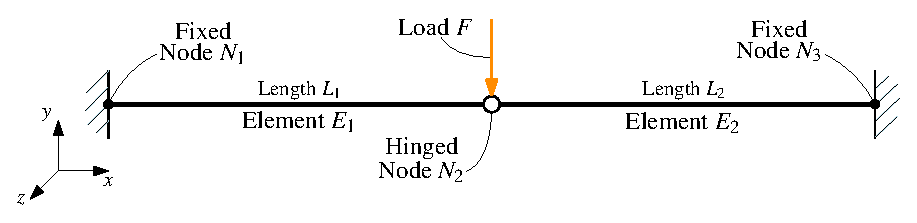
\includegraphics[width=0.7\textwidth]{./figures/chapter_7/usage_example.eps}
  \caption{Simple structure used to demonstrate the usage of the \TrussMe{} package.}
  \label{chap7:fig:usage_example}
\end{figure}

To describe the structure in \TrussMe{}, we first need to define the nodes. The nodes are defined using the \texttt{MakeNode} function
%
\begin{verbatim}
> N1 := MakeNode("N1", <0,0,0>, dofs=<0,0,0,0,0,0>):
> N2 := MakeNode("N2", <L_1,0,0>, dofs=<1,1,1,1,1,1>):
> N3 := MakeNode("N3", <L_1+L_2,0,0>, dofs=<0,0,0,0,0,0>):
\end{verbatim}
%
which takes as input the node name, the coordinates of the node, and the \acp{DOF}. In this case, the reference frames are not specified and the default ground frame, \ie{}, the identity matrix, is chosen for both nodes. The same is also for the \acp{BC} on displacements, which are not specified and are assumed to be zero. The \acp{DOF} are specified using a vector of six elements. The first three elements of the vector correspond to the displacements along and rotation around the $x$-, $y$-, and $z$-axes, respectively. The value of the \acp{DOF} can be either $0$ or $1$, where $0$ means that the \ac{DOF} is constrained to the ground and $1$ means that the \ac{DOF} is free. In this case, the nodes $N_1$ and $N_3$ are constrained in all directions, while the node $N_2$ is free. The modeling of the hinge on node $N_2$ is explained later in this section.

Before creating the elements, the material must be defined. Custom materials can be defined using the \texttt{MakeMaterial} function, which takes as input the material name, Young's modulus, Poisson's ratio, and density. If the shear modulus is not provided, it is computed from Young's modulus and Poisson's ratio. In this case, the material is defined as follows.
%
\begin{verbatim}
> M := MakeMaterial(name="GenericMaterial", elastic_modulus=E, shear_modulus=G,
    poisson_ratio=nu, density=rho):
\end{verbatim}
%
Then, the \texttt{MakeBeam} function is used, which requires the element's name, nodes at the element's ends, material, and cross-section properties.
%
\begin{verbatim}
> E1 := MakeBeam("E1", N1, [N2, <0,0,0,0,0,0>], material=M, area=A, inertia=[I_x,I_y,I_z],
    frame=GenerateFrameXY(N1["coordinates"], N2["coordinates"], [0,0,1])):
> E2 := MakeBeam("E2", [N2, <0,0,0,0,0,1>], N3, material=M, area=A, inertia=[I_x,I_y,I_z],
    frame=GenerateFrameXY(N2["coordinates"], N3["coordinates"], [0,0,1])):
\end{verbatim}
%
The reference frame of the element is also specified during the element definition. In this case, the reference frame is generated using the \texttt{GenerateFrameXY} function, which uses the coordinates of the two nodes to properly align the axes of the coordinate system. More information on how the element ends are linked to the nodes can be provided through an augmented vector of six elements, \eg{}, \texttt{[N, <1,1,1,1,1,1>]}. If the vector is not provided, the element ends are assumed to be rigid to the node in all directions. In the above code snippet, the element $E_1$ is connected to the node $N_1$ and to the node $N_2$ through a rigid connection. On the other hand, the element $E_2$ is hinged to the node $N_2$ by constraining the translational \acp{DOF} and leaving the rotational \acp{DOF} free. Lastly, the element $E_2$ is connected to the node $N_3$ through a rigid connection. In other words, the hinge connection is obtained by specifying the \acp{DOF} of the element ends that are free to rotate. In this case, the element $E_2$ is free to rotate around the $z$-axis.

Once the nodes and the elements are set, we can define the loads acting on the structure. The loads are defined using the \texttt{MakeLoad} function.
%
\begin{verbatim}
> F := MakeLoad("F", N2, <0,-P,0,0,0,0>):
\end{verbatim}
%
Also in this case, the load name, the node at which the load is applied, and the load magnitude are provided as input to the function. Optionally, the load reference frame can be specified using the \texttt{frame} parameter. If the reference frame is not specified, the node's reference frame is used. In this case, the load is applied to the node $N_2$ in the $y$-direction.

Finally, we can generate the \ac{FE} model of the structure using the \texttt{GenerateFEM} function and solve the linear system of equations using the \texttt{SolveFEM} function.
%
\begin{verbatim}
> fem := GenerateFEM([N1,N2,N3], [E1,E2], [F], tryhard):
> SolveFEM(fem, use_LEM=false, use_LAST=false):
\end{verbatim}
%
The \texttt{tryhard} flag enables the solvability check presented at (5b) step in the list above. If the user wants to use the \LEM{} and \LAST{} packages to solve the linear system of equations, the \texttt{use\_LEM} and \texttt{use\_LAST} flags must be set to \texttt{true}, in this case, the solution might be obtained in a veiled form. To force the unveiling of the solution, the \texttt{use\_LEM} flag must be set to \texttt{false}. After the solution of the linear system of equations is obtained, it is stored in the \texttt{fem} table.
%
\begin{verbatim}
> f = fem["f"]^%T; d = fem["d"]^%T;
\end{verbatim}
\begin{equation*}
  \begin{matrix}
    f = \left[\,\begin{matrix}
      \, 0, \, \dfrac{PL_2^3}{L_1^3+L_2^3}, \, 0, \, 0, \, 0, \, \dfrac{PL_1L_2^3}{L_1^3+L_2^3}, \, 0, \, -P, \, 0, \, 0, \, 0, \, 0, \, 0, \, \dfrac{PL_1^3}{L_1^3+L_2^3}, \, 0, \, 0, \, 0, \, -\dfrac{PL_1^3L_2}{L_1^3+L_2^3} \,
    \end{matrix}\,\right] \\[1.5em]
    d = \left[\,\begin{matrix}
      \, 0, \, 0, \, 0, \, 0, \, 0, \, 0, \, 0, \, \dfrac{PL_1^3L_2^3}{3EI_z(L_1^3+L_2^3)}, \, 0, \, 0, \, 0, \, \dfrac{PL_1^2L_2^3}{2EI_z(L_1^3+L_2^3)} \, 0, \, 0, \, 0, \, 0, \, 0, \, 0 \,
    \end{matrix}\,\right]
  \end{matrix}
\end{equation*}
%
For increased performance, the \TrussMe{} package is meant to be used alongside the \LEM{} and \LAST{} packages, which help control expression swell during the symbolic solution process. Further details on the usage of these packages can be found in \ref{chap7:sec:lem} and~\ref{chap7:sec:last} as well as in their respective documentation~\cite{lem2023source, last}. If both libraries are not available, the toolbox resorts to the \Maple{} built-in linear algebra routines.

If no symbolic solution can be found, or the user wants to evaluate the solution numerically, one can generate the \Matlab{} code using the \texttt{GenerateMatlabCode} function.
%
\begin{verbatim}
> GenerateMatlabCode("FemClass", fem, path="./dir/", info="Usage example class", vars=[P],
    data=[I_x=4.0e-4, I_y=2.0e-4, I_z=2.0e-4, E=210.0e6, nu=0.33, A=5.0e-3, L_1=1.0,
    L_2=1.0]);
\end{verbatim}
%
This function generates the \texttt{FemClass.m} file in the \texttt{./dir/} folder, containing a class definition of the just presented FE model. During the code generation process, the user can define default class properties in the \texttt{data} field, and variable parameters in the \texttt{vars} field. These latter are meant to be parameters that can change during the analysis of the structure, \eg{}, the load magnitude $P$. The details of the generated class and its usage are described in Section~\ref{chap7:subsec:numerical_computation}.

\subsection{The Numerical Computation in \Matlab{}}
\label{chap7:subsec:numerical_computation}

As the symbolic solution of~\eqref{chap7:eq:macrodf} is not always available, the user can resort to a numerical solution, which is obtained by numerical factorization of $\mathbf{K}^{n}_{ff}$ matrix and evaluation of~\eqref{chap7:eq:macrosol}. The numerical solution can be either obtained in the \Maple{} environment by variables substitution or in \Matlab{} after the code generation process. In the latter case, the \TrussMe{} \Matlab{} toolbox is used. The toolbox is based on the \texttt{TrussMe.System} base class that is used to define the components of~\eqref{chap7:eq:macrosol} and to provide a common framework to be exploited by the inherited classes. This abstract class contains several methods, some of which are virtual and must be implemented in the inherited classes: \\[0.5em]
%
\begin{minipage}[t]{0.49\textwidth}
  \begin{itemize}
  \setlength{\itemsep}{-0.25em}
  \item stiffness matrix $\mathbf{K}^{n}$;
  \item free-free stiffness matrix $\mathbf{K}^{n}_{ff}$;
  \item free-specified stiffness matrix $\mathbf{K}^{n}_{fs}$;
  \item specified-free stiffness matrix $\mathbf{K}^{n}_{sf}$;
  \item specified-specified stiffness matrix $\mathbf{K}^{n}_{ss}$;
  \item displacement vector $\mathbf{d}$*;
  \item free displacement vector $\mathbf{d}^{n}_{f}$*;
  \end{itemize}
\end{minipage}
\hfill
\begin{minipage}[t]{0.49\textwidth}
  \begin{itemize}
  \setlength{\itemsep}{-0.25em}
  \item specified displacement vector $\mathbf{d}^{n}_{s}$;
  \item force vector $\mathbf{f}$*;
  \item free force vector $\mathbf{f}^{n}_{f}$;
  \item specified force vector $\mathbf{f}^{n}_{s}$*;
  \item remainder force vector $\mathbf{f}^{n}_{r}$;
  \item \acp{DOF} permutation $\mathbf{P}^{n}$;
  \item getters and setters for the system data;
  \end{itemize}
\end{minipage} \\[0.5em]
%
where (*) means that it is available only if the system symbolic solution is available, otherwise an empty vector is returned.

\subsubsection*{\TrussMe{} Numerical Computation Usage Example}

The \TrussMe{} \Matlab{} toolbox is used to evaluate the solution of the problem numerically. The usage of the toolbox is quite straightforward if the code is generated through the \TrussMe{} \Maple{} package. Let us suppose that we have generated the \texttt{FemClass.m} file using the \TrussMe{} \Maple{} package. This file contains the class definition of the structure. To use the generated class, we first need to instantiate it.
%
\begin{verbatim}
>>> fem = FemClass();
\end{verbatim}
%
Optionally, we can set the value of the internal data of the class during the instantiation.
%
\begin{verbatim}
>>> data.I_x = 4.0e-4; data.I_y = 2.0e-4; data.I_z = 2.0e-4; data.E = 210.0e9; ...
    data.A = 5.0e-3; data.L_1 = 1.0; data.L_2 = 1.0;
>>> fem = FemClass(data);
\end{verbatim}
%
We can either set or get the value of the internal data of the class after the instantiation or by using the dedicated methods.
%
\begin{verbatim}
>>> fem.set_data_field('I_x', 4.0e-4);
>>> I_x = fem.get_data_field('I_x');
>>> fem.set_data(data);
>>> data = fem.get_data();
\end{verbatim}
%
After instantiation, the components of the system of equations~\eqref{chap7:eq:macrosol} can be obtained using the following methods.
%
\begin{verbatim}
>>> x = [1000];
>>> v = fem.v(x);
>>> d = fem.d(x,v);
>>> f = fem.f(x,v);
\end{verbatim}
%
Notice that the vector \texttt{x} contains the parameters of the system, \eg{}, the load value $P$ of \SSI{1000}{\newton}, and the vector \texttt{v} the values of the veiling variables that may have been stored during the computation of the symbolic solution according to \ref{chap7:sec:lem} and \ref{chap7:sec:last}. If the symbolic solution is not available, it can be numerically calculated.
%
\begin{verbatim}
>>> x = [1000];
>>> v = fem.v(x);
>>> d = fem.compute_d(x,v);
>>> f = fem.compute_f(x,v);
\end{verbatim}
%
The least squares solution can be also obtained by adding the tolerance value and the maximum number of iterations to the \texttt{compute\_d} and \texttt{compute\_f} methods, \eg{}, \texttt{fem.compute\_f(x,v,tol,iter)}. Other numerical solution methods based on the constrained minimization of energy functional can be used to solve the system of equations~\eqref{chap7:eq:macrosol}~\cite{hutton2004fundamentals}. However, these methods are not implemented in the \TrussMe{} \Matlab{} toolbox.

% % % % % % % % % % % % % % % % % % % % % % % % % % % % % % % % % % % % % % % %

\section{Example Applications}
\label{chap7:sec:example_applications}

In this section, we briefly present two example applications of the \TrussMe{} toolbox. In all the examples, the rear left double wishbone suspension of the Formula SAE \emph{E-Agle Trento Racing Team} (\emph{University of Trento}) vehicle~\citep{eagle} is considered. The suspension is represented in Figure~\ref{chap7:fig:suspension} where, on the left-hand side, the rendering of the system is displayed along with the names of the main components, and on the right-hand side, the schematic representation of the suspension system is reported. In the following paragraphs, we will see how the \TrussMe{} toolbox can be used to perform the design optimization of the suspension system and to efficiently include the kinematics and compliance of the suspension system through model reduction. The results obtained with the \TrussMe{} toolbox are validated with the results obtained using the commercial software \Ansys{}. Notice that the in-depth discussions on the results of the example applications tests are available in~\cite{larcher2024symbolic}.

Before proceeding with the example applications, it is important to make clear that in this case, the \TrussMe{}'s package is used to symbolically assemble the structure and simplify the expressions of the linear system components. Then, the symbolic code is exported in the \Matlab{} class by specifying the internal data and the input parameters of the system. The \Matlab{} class is then used to evaluate the solution of the problem numerically in the \Simulink{} environment. This approach is necessary since the symbolic kernel is significantly slowed down by the size and complexity of the arising linear system.

\begin{figure}[!ht]
  \centering
  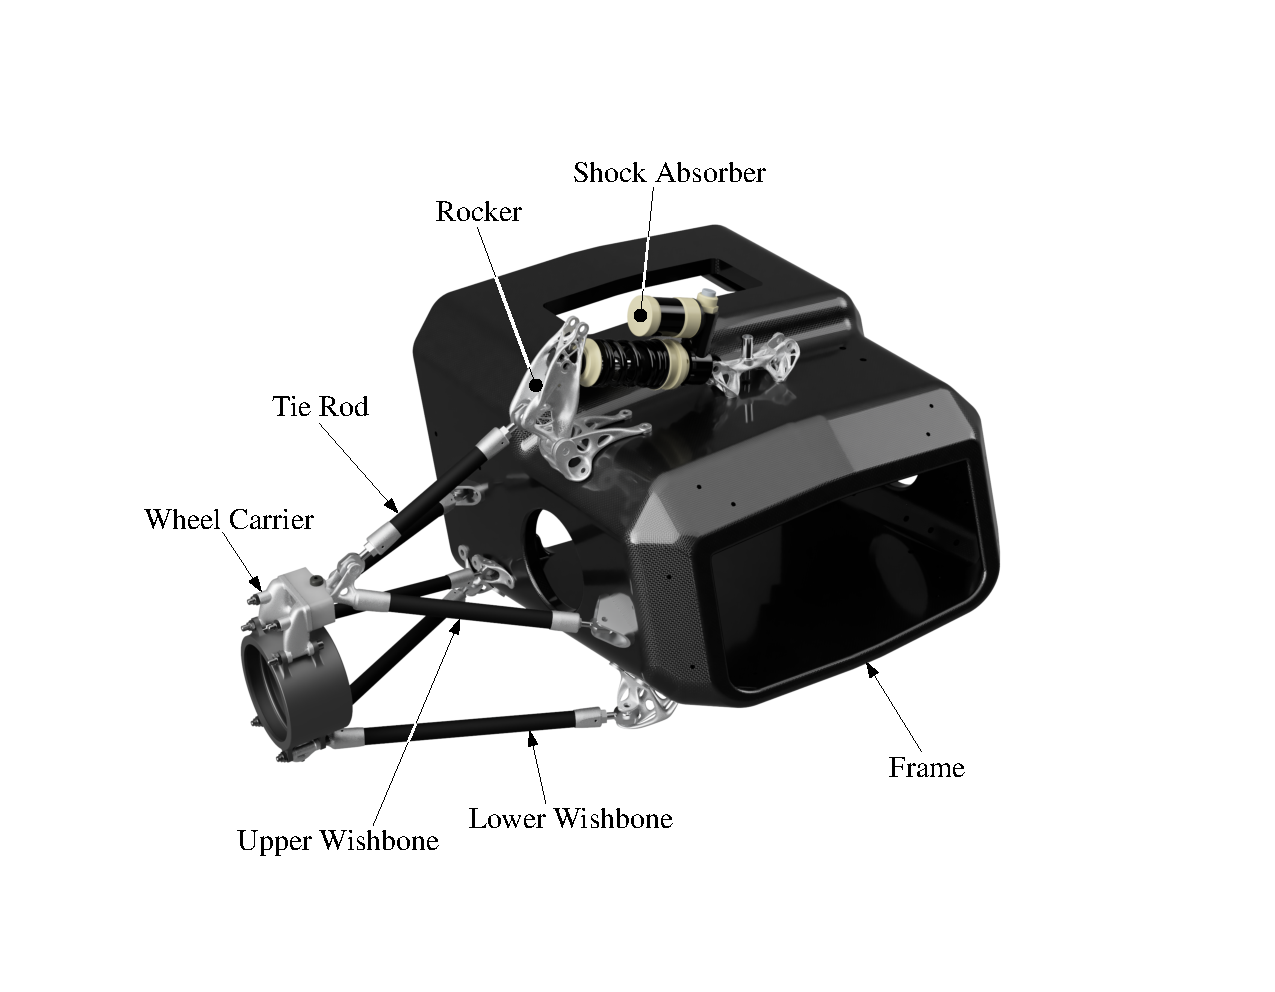
\includegraphics[width=0.5\textwidth, trim={2cm 2cm 2.5cm 2cm}, clip]{./figures/chapter_7/rendering.eps}
  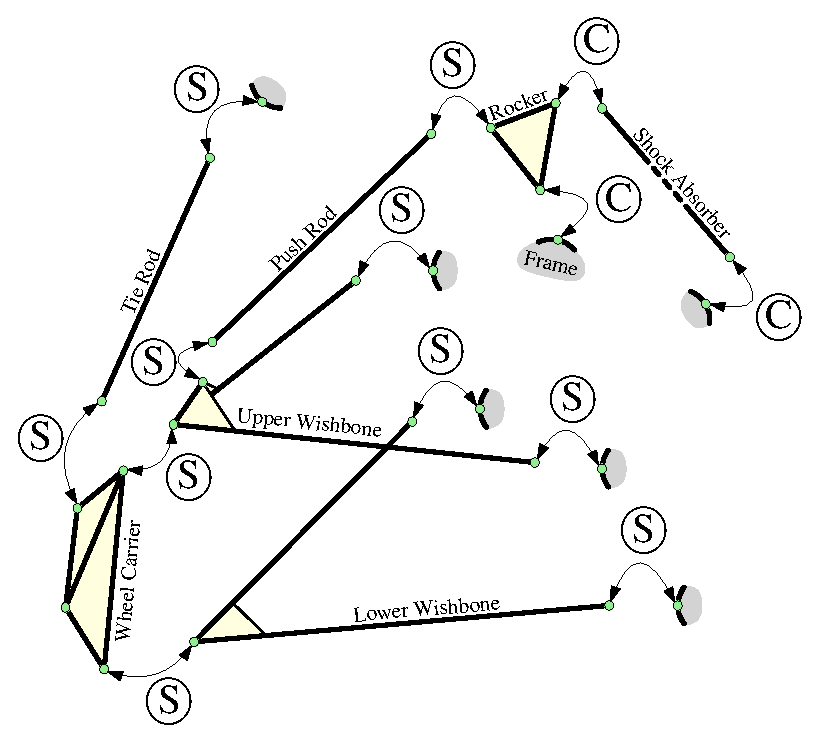
\includegraphics[width=0.4\textwidth]{./figures/chapter_7/constraints.eps}
  \caption{Rendering and schematic representation of the rear left double wishbone suspension. The spherical and cylindrical constraints are respectively represented by the symbols \circled{S} and \circled{C}.}
  \label{chap7:fig:suspension}
\end{figure}

\subsection{Design Optimization}

Moving mechanisms are widely used in engineering applications. Typically, the design of these mechanisms is performed assuming rigid bodies. However, in certain cases, the flexibility of the mechanism can have a significant impact on the performance of the mechanism. Optimization is a powerful tool that can be used to design structures with optimal performance. The \TrussMe{} toolbox can be used to perform shape optimization to both reduce the compliance of the mechanism and minimize the internal forces. Specifically, the goals of the presented optimizations are to minimize the wheel compliance hub angle $\theta_z$ and the tie rod axial force $F_a$ by varying the $x$- and $z$- coordinates of the hard point connecting the tie rod to the chassis, which according to~\cite{larcher2024symbolic} is referred to as the point $P_5$. The results of both optimizations are reported in~\figurename{}~\ref{chap7:fig:optimization}. These optimization examples show that the current design does not represent the optimal solution in terms of both minimum tie rod axial force and minimum wheel compliance hub angle. The optimum conditions are achieved by the combination of the values indicated by the green point. It is worth noting that the presented optimizations serve only as a proof of concept of the model's parametric characteristics. In a real case scenario, a multi-objective optimization should be performed taking into consideration the compliance and structural analysis along with the kinematic characteristic of the suspension.

\begin{figure}[!ht]
  \centering
    \begin{subfigure}[t]{0.49\textwidth}
    \small{\includetikz{./figures/chapter_7/optimization_hub_angle.tex}}
    \caption{Wheel hub compliance angle $\theta_z$ dependency from the $x$- and $z$- coordinates of the $P_5$ hard point.}
    \label{chap7:fig:variation_theta_z}
  \end{subfigure}
  \hfill
  \begin{subfigure}[t]{0.49\textwidth}
    \centering
    \small{\includetikz{./figures/chapter_7/optimization_tie_force.tex}}
    \caption{Tie rod axial force $F_a$ dependency from the $x$- and $z$- coordinates of the $P_5$ hard point.}
    \label{chap7:fig:variation_force_tie}
  \end{subfigure}
  \caption{Optimization of the point $P_5$ $x$- and $z$- coordinates to minimize the wheel compliance hub angle $\theta_z$ and the tie rod axial force $F_a$. The tests are performed by applying a constant $M_z$ torque of \SSI{0.4}{\kilo\newton\meter}. \emph{Marks legend:} {\color{mycolor2}\raisebox{-.15pt}{\Large$\bullet$}} current design, {\color{mycolor5}\raisebox{-.15pt}{\Large$\bullet$}} optimality condition.}
  \label{chap7:fig:optimization}
\end{figure}

\begin{figure}[htp!]
  \centering
  \small{\includetikz{./figures/chapter_7/suspension_static_deformations.tex}}
  \caption{Comparison of the displacements and rotations of the wheel carrier reference frame in and around the $x$-, $y$-, and $z$-axes for different loads applied at the wheel hub obtained using the \TrussMe{} toolbox (\emph{lines}) and the \Ansys{} finite element analysis software (\emph{dots}). On the left-hand side of the figure, the forces are applied and torques are null. Conversely, the right side of the figure reports the results where torques are applied and forces are null.}
  \label{chap7:fig:suspension_static_results}
\end{figure}

\begin{figure}[!ht]
  \centering
  \begin{minipage}[c]{0.575\linewidth}
    \small{\includetikz{./figures/chapter_7/suspension_dynamic_deformations.tex}}
  \end{minipage}
  \begin{minipage}[c]{0.125\linewidth}
    \vspace{-2.5em}
    \begin{center}
      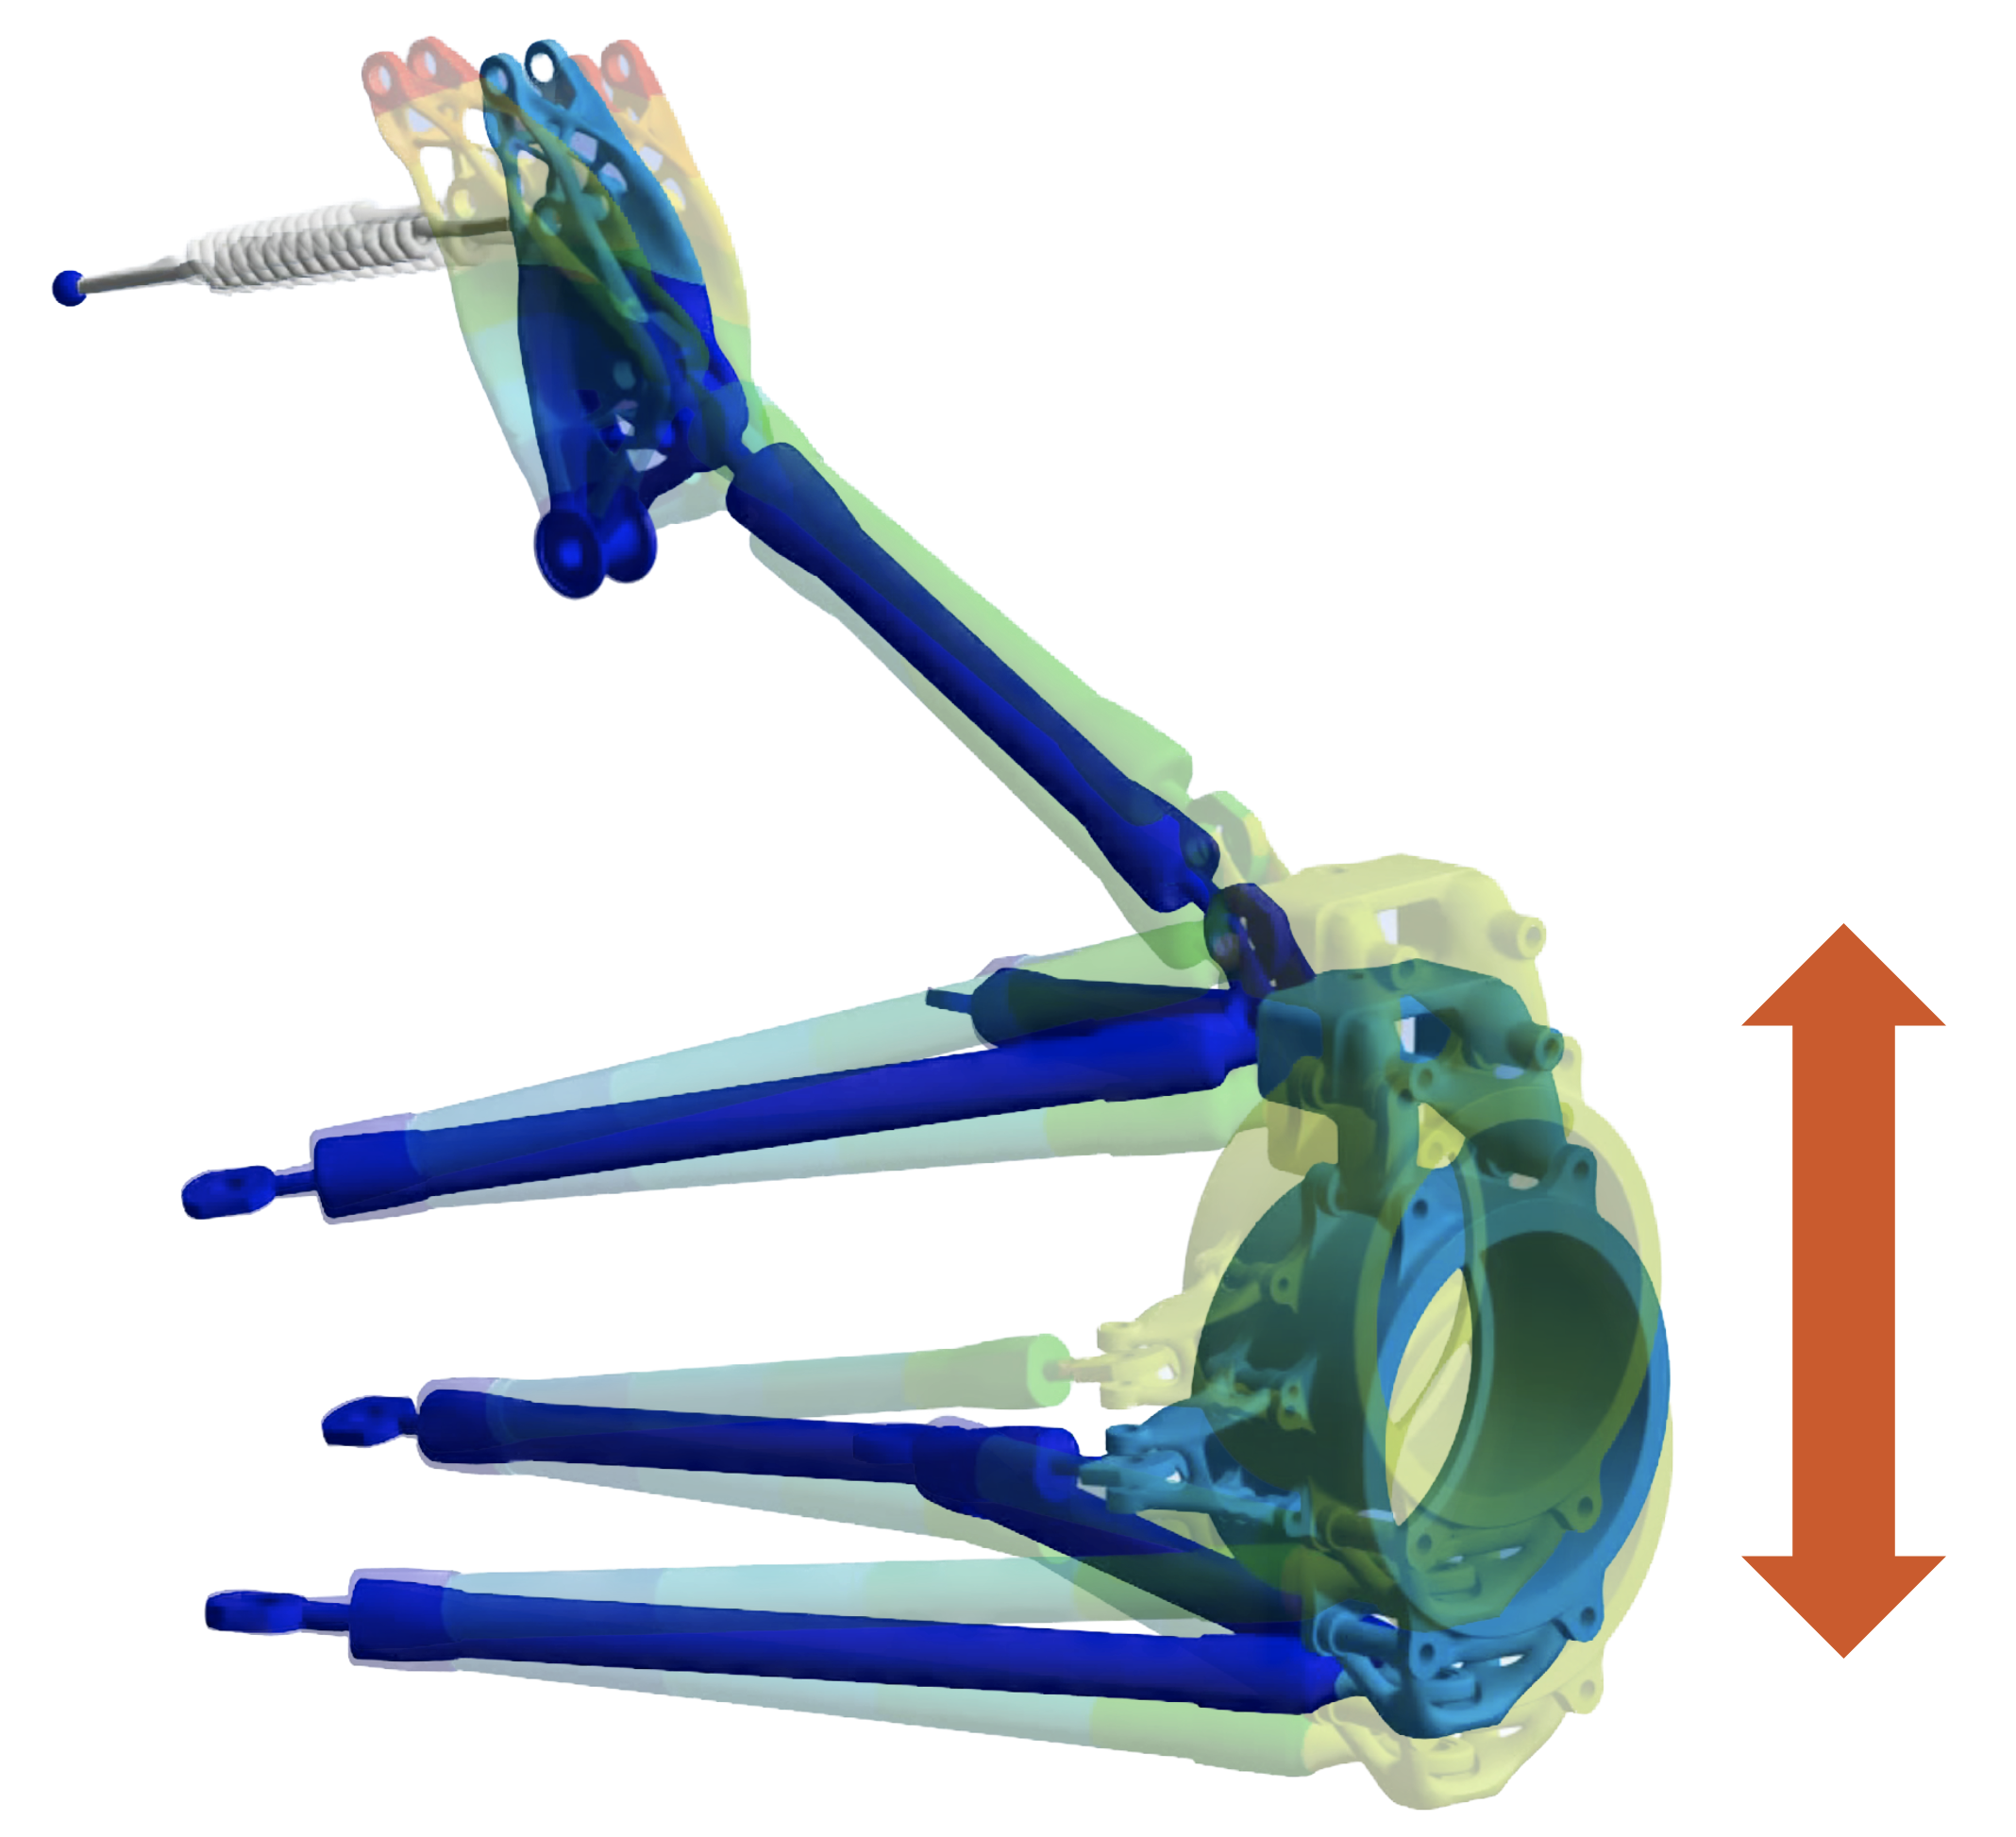
\includegraphics[width=1.0\linewidth]{./figures/chapter_7/mode1.png} \\ \small{$f_1 = \SSI{7.6}{\hertz}$} \\[0.8in]
      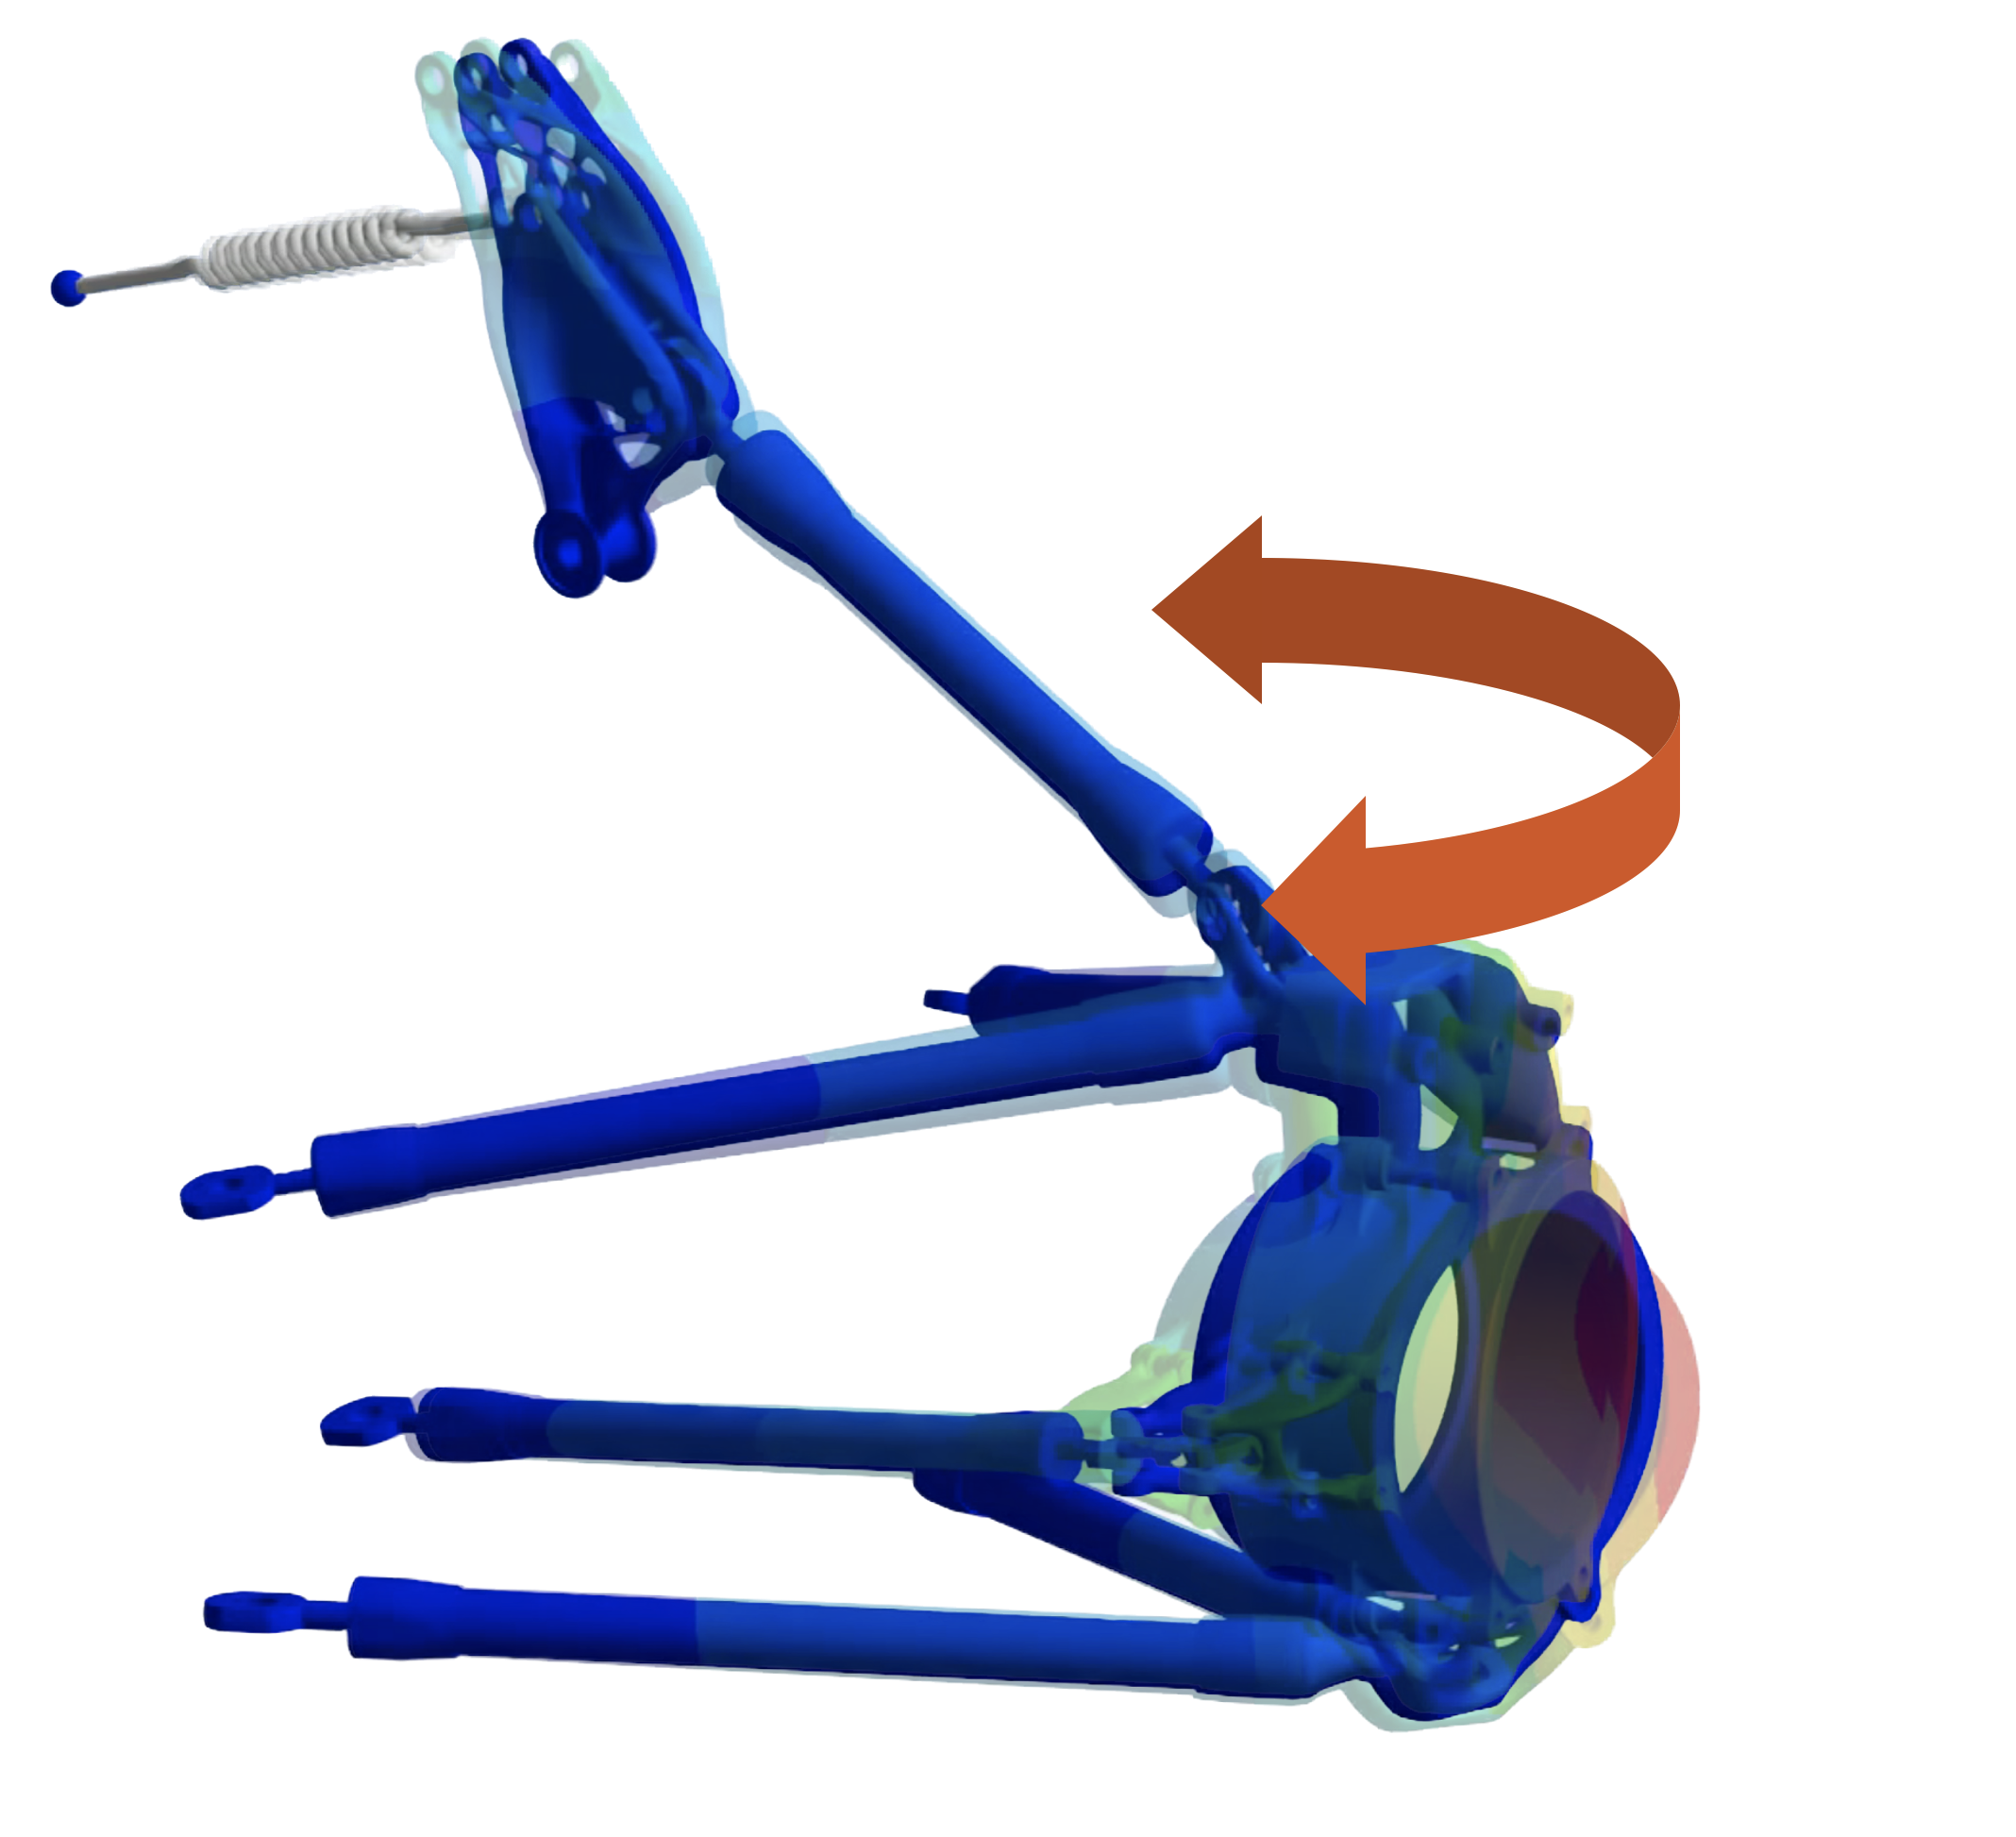
\includegraphics[width=1.0\linewidth]{./figures/chapter_7/mode2.png} \\ \small{$f_2 = \SSI{88.5}{\hertz}$} \\[0.8in]
      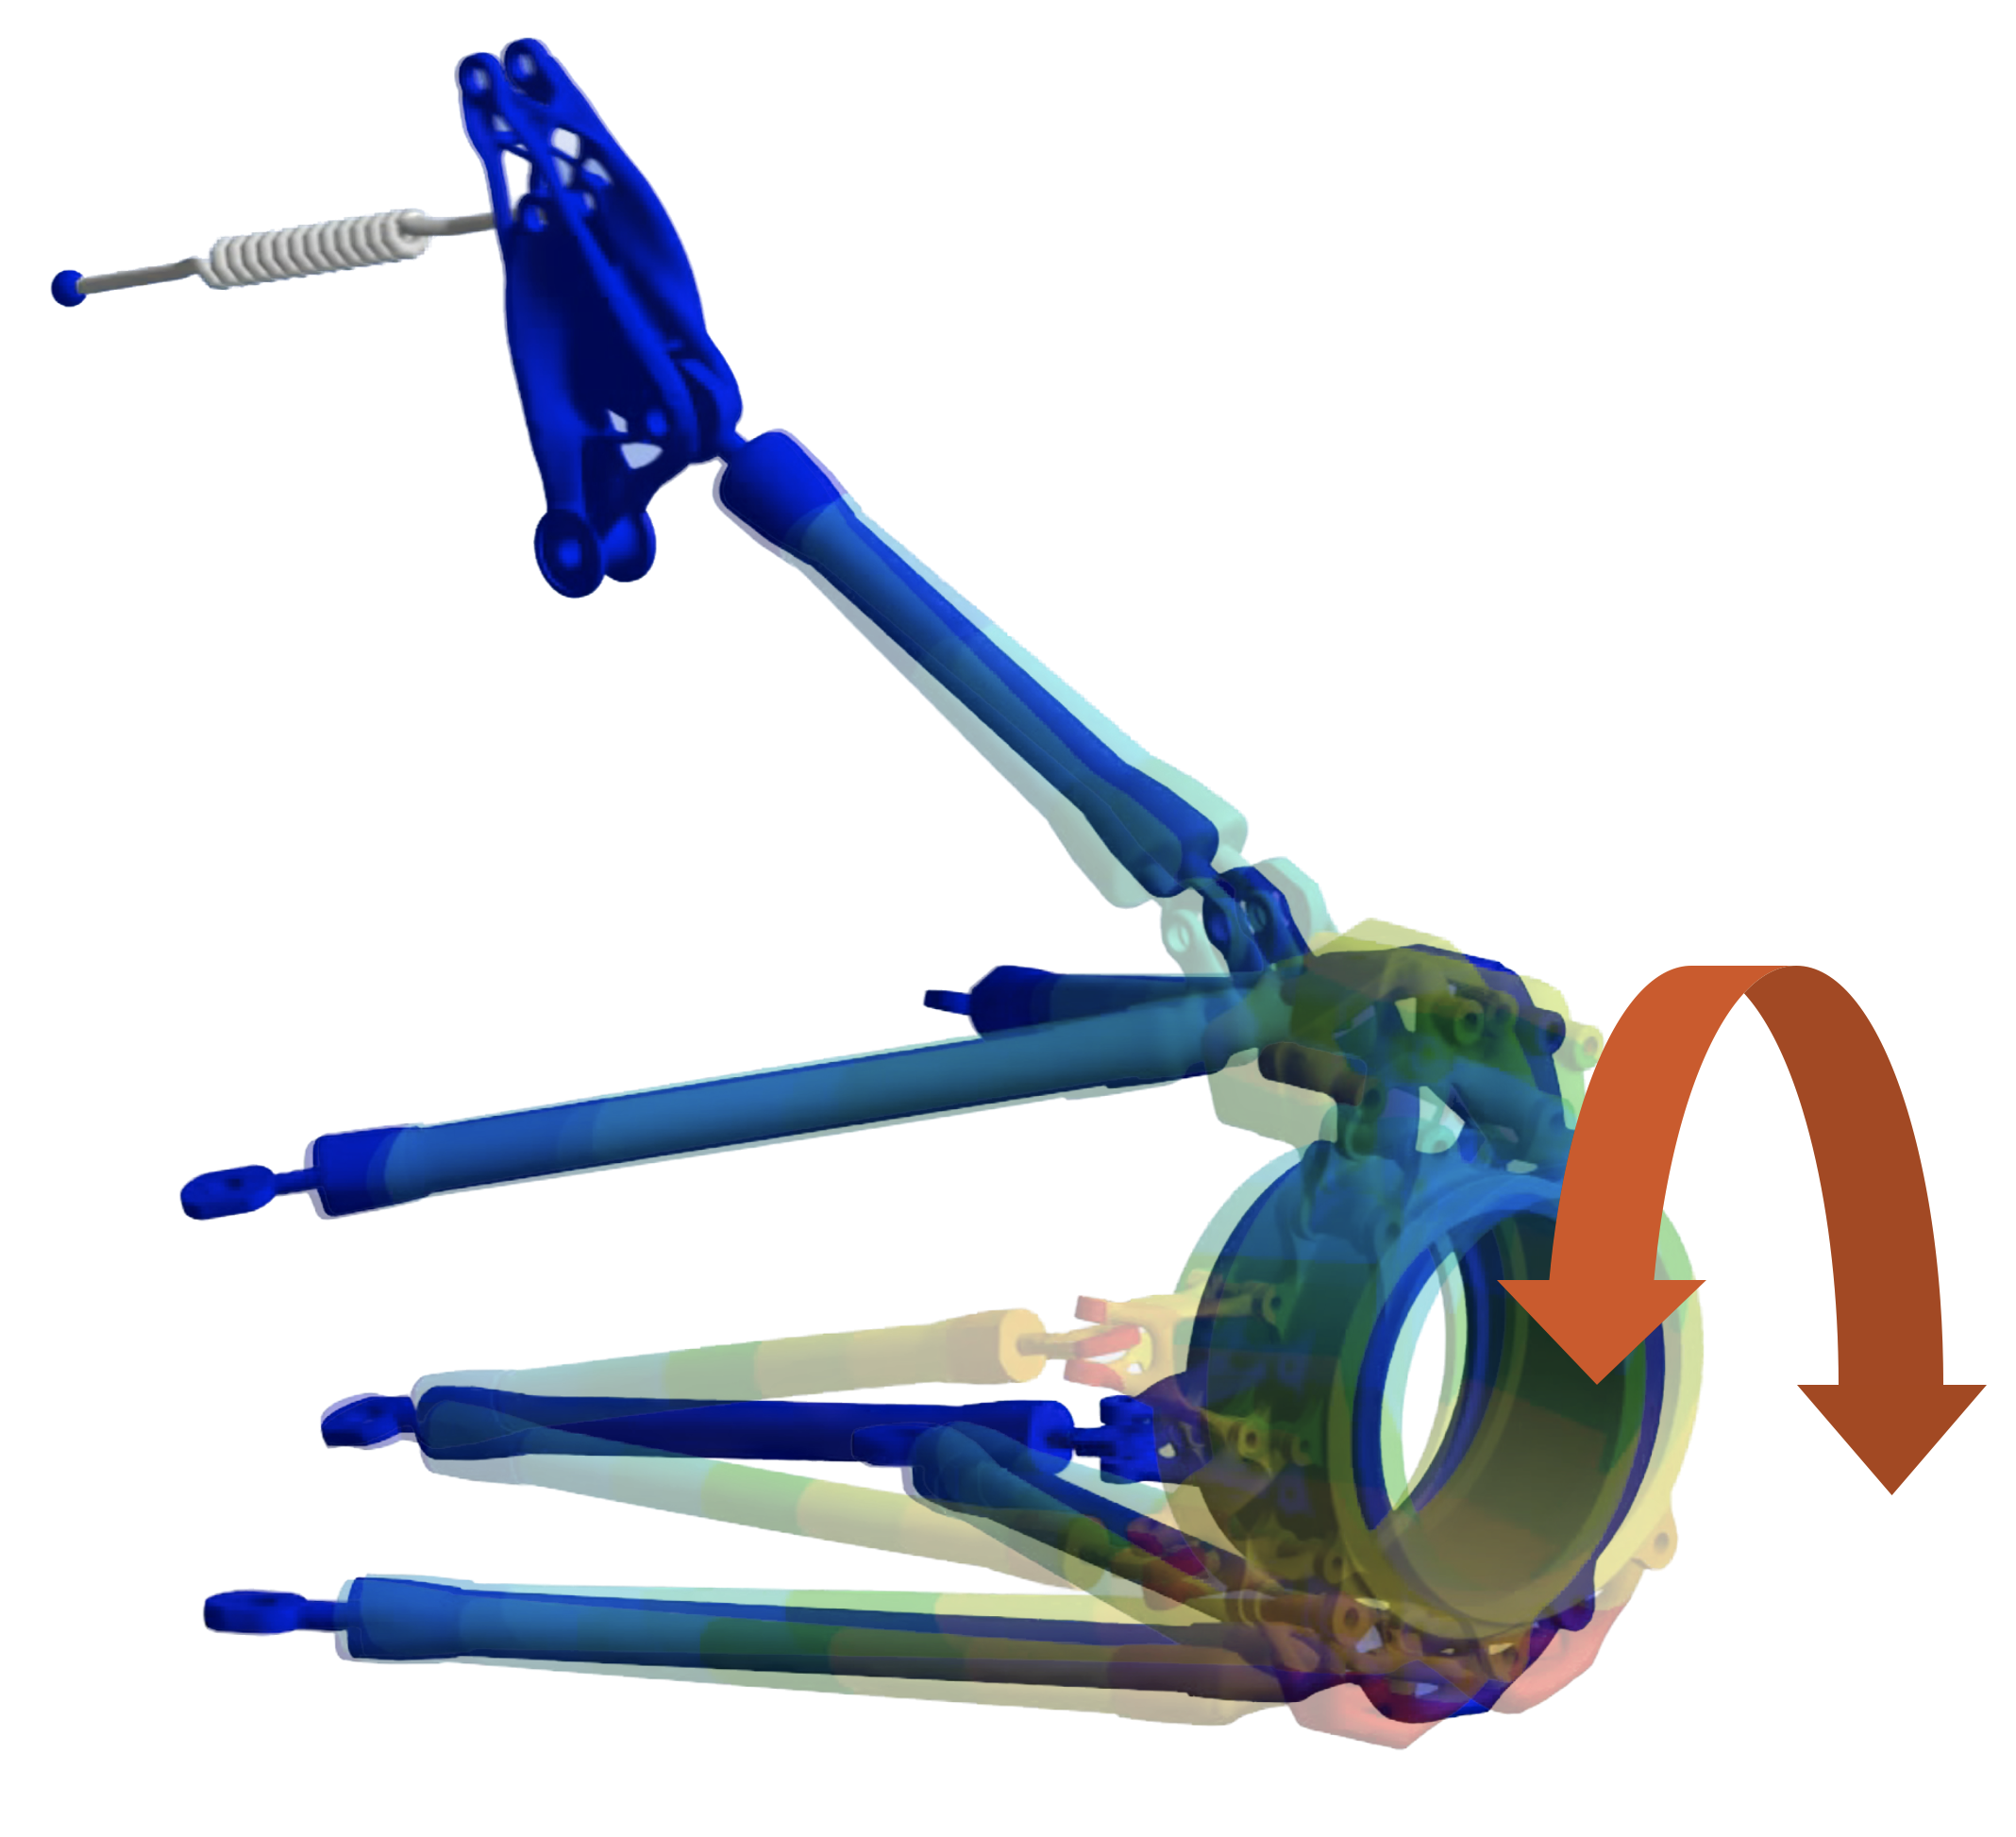
\includegraphics[width=1.0\linewidth]{./figures/chapter_7/mode3.png} \\ \small{$f_3 = \SSI{159.7}{\hertz}$} \\
    \end{center}
  \end{minipage}
  \caption{Frequency response analysis of the suspension model. The tests are performed under the equilibrium between the suspension system and a vertical force of \SSI{500}{\newton} applied at the wheel hub. The frequency responses are evaluated by applying input forces/torques at the wheel hub as a linear chirp with a frequency in the range \RSI{0}{200}{\hertz} and a constant amplitude of \SSI{5}{\newton}/\SSI{5}{\newton\meter}. Next to the Bode plots, on the right-hand side, the first three modal shapes of the suspension are illustrated along with their corresponding frequency. \emph{Legend:} {\color{mycolor1}$\blacksquare$} \Simulink{} multi-body simulation with full compliance dynamics contribution, {\color{mycolor2}$\blacksquare$} \Simulink{} multi-body with steady-state compliance contribution, {\color{mycolor3}$\blacksquare$} \Ansys{} \ac{FE} modal analysis}
  \label{chap7:fig:suspension_dynamic_results}
\end{figure}

\subsection{Efficient Simulation of Parametric Mechanisms Using Model Reduction}

This example application is used to the explore inclusion of suspension compliance in the simulation of a vehicle using a hybrid symbolic-numerical approach. This methodology allows for easy generalization and run-time modification of the model parameters without the requirement to regenerate code. The dynamic characteristic of the suspension is modeled through a differential-algebraic equation system, which is integrated by the methods described in~\cite{larcher2024symbolic}. Depending on the modeling approach, suspension pick-up points' position and tire force at the hub are either extracted by a semi-analytical solution or by numerical integration and then used to calculate the compliance characteristics of the suspension. The compliance contribution can be included in the overall displacement of the suspension system as a \emph{steady-state} or \emph{full dynamic} contribution~\cite{larcher2024symbolic}. The first approach is used to reduce the computational cost of the simulation, while the latter leads to accurate simulations at a higher computational cost. The results of the presented approach are compared with the simulation data obtained using commercial software \Ansys{} and show good agreement in both static (\figurename{}~\ref{chap7:fig:suspension_static_results}) and dynamic conditions (\figurename{}~\ref{chap7:fig:suspension_dynamic_results}).

% % % % % % % % % % % % % % % % % % % % % % % % % % % % % % % % % % % % % % % %

\section{Conclusions}
\label{chap7:sec:conclusion}

In this paper, we have presented the \TrussMe{} toolbox, a symbolic-numerical toolbox for the analysis of structures. The toolbox is based on the \ac{DSM} and it is proven to be a valuable tool for modeling, simulation and optimization of structures. The toolbox is composed by two parts: the symbolic manipulation part and the numerical evaluation part. The symbolic part is implemented as \Maple{} package and it performs the assemblage and simplification of the linear system of equations. Code generation exports the symbolic code in a \Matlab{} class. The numerical part is implemented in \Matlab{} and it is used to evaluate the solution of the problem numerically if the symbolic solution is not available. The \TrussMe{} toolbox is validated through two example applications. Lastly, the difficulties in the computation of the symbolic solution of the linear system of equations are mitigated by the \LEM{}~\cite{lem} and \LAST{}~\cite{last} \Maple{} packages, which are presented as optional tools to be used alongside the \TrussMe{} toolbox.

% % % % % % % % % % % % % % % % % % % % % % % % % % % % % % % % % % % % % % % %
